\chapter{Struttura progetto}\label{cap:struttura}
Il progetto è stato strutturato seguendo un approccio simile all'\var{MVC}\footnote{Model-View-Controller}, in particolare è stata realizzata un'architettura suddivisa in tre livelli principali:
\begin{description}
\item[View:] Riguarda la parte che interagisce con l'utente, ovvero l'interfaccia grafica e l'interfaccia web.
\item[Controller:] Questo livello contiene tutte le classi che vengono utilizzate per consentire al livello view di richiamare le funzionalità del software.
\item[Model:] Quest'ultimo livello contiene il cuore del progetto, che a sua volta può essere suddiviso in vari sottolivelli.
\end{description}
\begin{figure}[htb]
\begin{center}
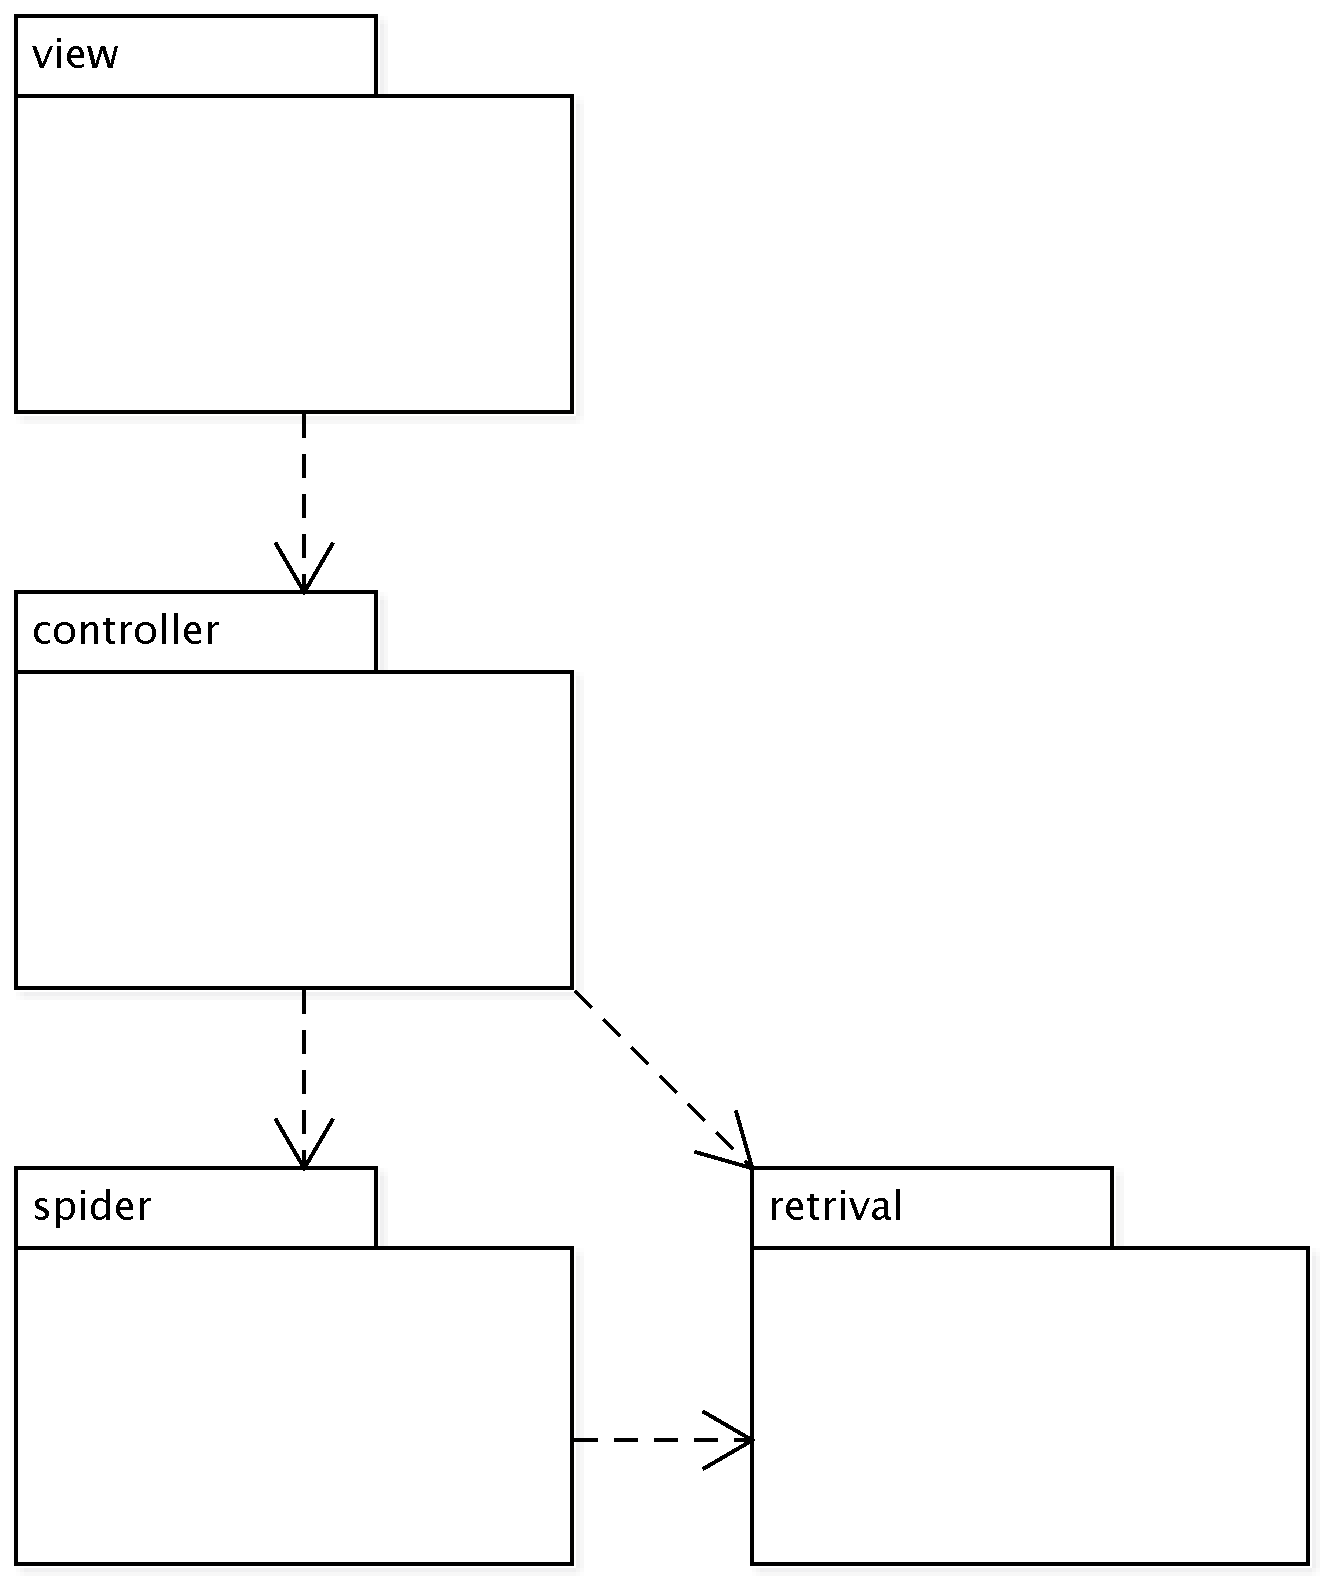
\includegraphics[scale=0.10]{etc/architettura.png}
\caption{Architettura}
\label{architettura}
\end{center}
\end{figure}
\section{Model}
Tale livello contiene le due parti fondamentali del software realizzato, che sono lo \var{spider} e il modulo di \var{retrival}. Il tutto è stato realizzato mantenendo la più alta modularità ed astrazione possibile, in modo da rendere semplice la manutenzione.
\subsection{Spider}
Intuitivamente lo Spider potrebbe sembrare la parte più complessa del software, in realtà vi si è stato speso poco tempo rispetto al resto del progetto; questo perchè è stato utilizzato uno Spider già esistente, in particolare \var{Websphinx}\footnote{\url{http://www.cs.cmu.edu/$\sim$rcm/websphinx/}}. Il lavoro speso sullo Spider si è incentrato sulla sua documentazione, e sul realizzare le nostre API di più alto livello, per una semplice gestione dello Spider. Inoltre si è fatto in modo che lo Spider si comporti come Thread consentendo al resto dell'applicazione di continuare ad operare, evitando delle lunghe attese dovute alla latenza dello spidering. Realizzando quanto appena detto è possibile interagire con lo Spider anche durante lo spidering, il che permettere di effettuare delle richieste tra cui: il numero di pagine recuperate, le pagine recuperate, interrompere lo spidering e avviare una nuova scansione.
\subsubsection{SpiderExplorer}
Come precedentemente detto è possibile recuperare le pagine esplorate, per realizzare tale lavoro è stato progettato un modulo chiamato \var{SpiderExplorer} che consente la navigazione dei risultati ottenuti dalla ricerca di quelli che si attengono al Task richiesto\footnote{Un task potrebbe essere ``Università Tor Vergata''}. Tale modulo effettua inoltre un operazione di indicizzazione sulle pagine, sfruttando il modulo di \var{Retrival}.
\subsection{Retrival}
Questo modulo consente la gestione del sistema di indicizzazione e di retrival di \var{Lucene}, infatti rende possibile indicizzare nuovi documenti (nel nostro caso informazioni sulle pagine recuperate) ed effettuare delle ricerche sui documenti presenti nell'indice. Questo come già accennato viene sfruttato dallo Spider per filtrare le pagine che si attengono al task da quelle che non sono rilevanti. Inoltre sono state aggiunte delle funzionalità che consentono l'espansione delle query tramite Rocchio e Wordnet. In seguito verranno discussi approfonditamente i moduli elencati.
\section{Controller}
Il Controller consente di gestire tutte le funzionalità dello Spider e del modulo di Retrival, in particolare sarebbe un livello di astrazione più elevato che consente al livello successivo, ovvero View, di gestire tutto il software tramite l'ausilio di qualche semplice istruzione.
\section{View}
Questo layer potrebbe sembrare non molto rilevante, invece è risultato essere uno dei più complessi da realizzare. Tale difficoltà si è incontrata a causa della necessaria interazione tra l'applicazione desktop e l'applicazione web. Infatti per consentire una comoda navigazione dei risultati delle ricerche sono state progettate due interfacce grafiche, una web ed una desktop. La prima è molto più comoda per navigare tra i risultati all'interno del task, ad esempio con task = ``Tor Vergata'' ed una query = ``Ingegneria''. L'interfaccia desktop invece è stata strutturata per consentire una semplice ed intuitiva navigazione delle pagine esplorate dallo Spider che si attengono al task, il tutto grazie ad un grafo esplorabile con il mouse.